\noindent
In this section we systematically study the effect of topology of the underlying contact network on the broadcast time and wastage and come up with some suggestions which we 
feel will be helpful while designing networks.  
%First we analyze the B-P algorithm on complete graph topology and observe that the broadcast time scales 
%as $n^{\frac{k-1}{k}}$. 
We first analyze B-P algorithm on different topologies like regular graph, regular tree and random graph. In particular, we wish to 
check whether the average degree ($d$) of the underlying contact network influences the 
 performance metrics. 
 %Since it is difficult to interpolate through every value of $d$ for a real network, we perform our simulations on the synthetic networks.
 In the later part of this section we make a comparative study of different broadcast strategies (discussed in section ~\ref{algorithm_outline}) and also
 reinspect into their sparser variants to identify the effect of lowering the value of $d$ 
 through removal of edges without hampering network connectivity.
\subsection{Blind push on different topologies} 
\if{0}
%\vspace{-5mm}
\subsection{Blind push on complete graph}
% \vspace{-2mm}
 We analyze the performance of B-P on complete graph topology. A complete graph topology indicates that a node in the system can communicate with any other node. 
 We provide numeric evidence (with analytical support) that the
ratio of the overall broadcast time $T^{\ast }$ and the time to
create the first sender, i.e., $T_{1}$ converges to a constant which only depends on $k$. 
For this purpose we plot in figure~\ref%
{segSizeVsDelay_nrTrans_varyN_Mall_push_pull} the values of $Av(T^{\ast })$
and $Av(T_{1})$ respectively as we vary $n$ where $Av(y)$ represents the average of the quantity $y$ over several simulation runs. We report this distribution for
four different values of $m$ (2, 4, 8 and 16), in each case assuming that
there is only one message segment, i.e., $k=m$. Note that for B-P, the two quantities $Av(T^{\ast })$ and $Av(T_{1})$
exhibit a very similar profile irrespective of the value of $m$ chosen. In the same figure we also plot the function $n^{\frac{k-1}{k}}$ suitably scaled by a constant to show how the theoretical results which we provide next, closely approximate the numerical simulations. 

\begin{figure}[htbp] 
\centering
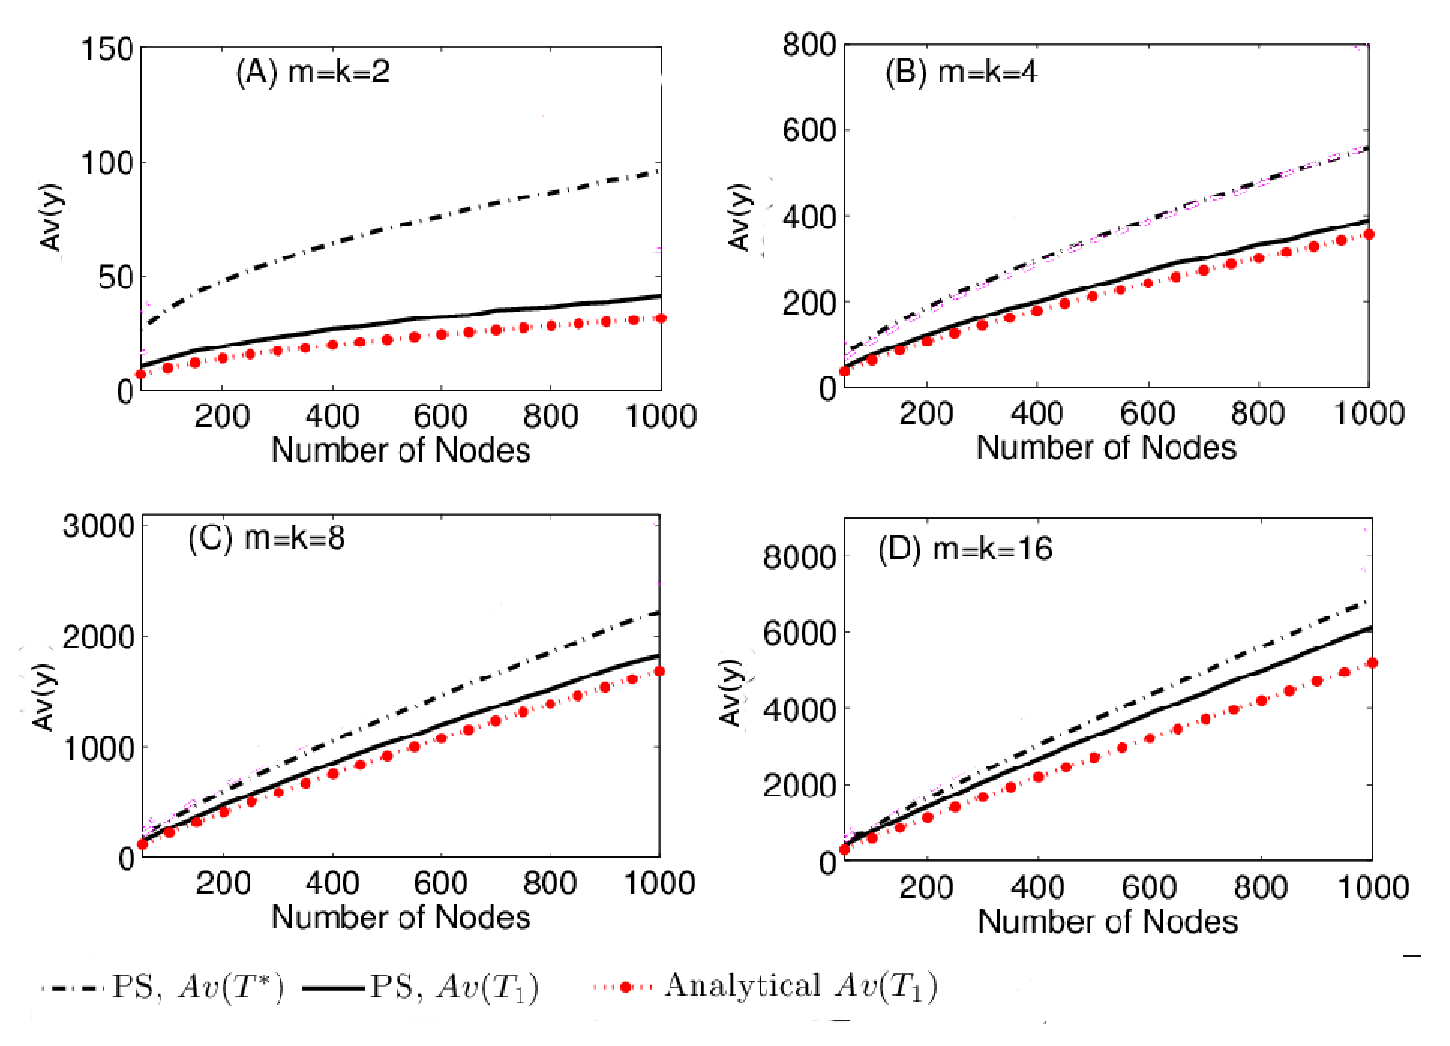
\includegraphics[scale=0.36]{./texfiles/Chapter_3/netsci/figs1/segSizeVsDelay_nrTrans_varyN_Mall_push_pull2.eps}
\caption{$Av(T^*)$ and $Av(T_1)$ versus the number of nodes ($n$). Results are presented for (A) $m=k=2$, (B) $m=k=4$, (C) $m=k=8$, and (D) $m=k=16$. The plots also contain the suitably scaled function $n^{\frac{k-1}{k}}$ for each case.}
\label{segSizeVsDelay_nrTrans_varyN_Mall_push_pull}
\end{figure}
%\subsection{Performance of B-P in the limit $n\rightarrow \infty$ for complete graph topology}
\subsubsection{Analytical estimate}

We initially start by considering a message which has $m=2$ packets and $s=1$ segment (i.e., the segment has $k=2$ packets). We compute the expected time to 
obtain the first sender\footnote{
Note that first sender refers to the first node (other than the initiator) which 
receives the full message during the broadcast phase.
} $E(T_1)$. 
%and the expected time for broadcast $E(T^{\ast})$. 
It is important to note that $T_1$ is an indicator for the total broadcast time $T^*$ since the remaining growth is of logarithmic order as after creation of the first sender, 
several senders are produced at regular interval thus speeding
up the transfer exponentially. 
We provide an outline of the analytical expression, the detail is more involved and is ommitted in the interest of space. 
 
At time $T_0$, an initiator is created and it has the full message. Since we are considering 
message size of $2$ so the first sender can be created at least in 2 time steps which is possible
 if the same node is selected in these two time steps. Next we calculate 
$Pr\{T_1=t\}$ that is the probability that the  first sender is created at time $t$. This implies
for the $t-1$ time steps, only the nodes without any packets are selected and at time step $t$ one 
from the $t-1$ nodes are selected. So we have


\begin{align*}
\Pr \{ T_{1}=t\} &=(1-\frac{1}{n})(1-\frac{2}{n})(1-\frac{3}{n})...(1-\frac{t-2}{n})(\frac{t-1}{n}) \\ 
 &=\frac{t-1}{n}\prod\limits_{l=1}^{t-2}( 1-%
\frac{l}{n}) ,t\geq 2
\end{align*}
Infact if $\tau_i$ represent the time to create the first sender then it can be shown that the recursion  $\frac{E\left( \tau _{i}\right) }{E\left(
\tau _{i-1}\right) }=\left( 1-\frac{3}{2i}\right) $ holds. 
From this one can show that $E(T^*)=2*E(T_1)$
\if{0}
Writing $\left( 1-\frac{l}{n}\right) =e^{-\frac{l}{n}+O\left( \frac{l^{2}}{%
n^{2}}\right) }$we have for the cumulative distribution function 
\begin{eqnarray*}
\Pr \left\{ \frac{t_{1}}{\sqrt{n}}\leq x\right\}  &=&\sum\limits_{t\leq x%
\sqrt{n}}\frac{t-1}{n}\prod\limits_{l=1}^{t-2}\left( 1-\frac{l}{n}\right)  \\
&=&\sum\limits_{t\leq x\sqrt{n}}\frac{t}{n}e^{-\frac{t^{2}}{2n}+O\left( 
\frac{t^{3}}{n^{2}}\right) }
\end{eqnarray*}%
For $n\rightarrow \infty $, the sum in the last expression converges to $%
\int\limits_{0}^{x}ye^{-\frac{y^{2}}{2}}dy.$  Hence the limiting density is
given by $ye^{-\frac{y^{2}}{2}}$ and the expectation by $\int\limits_{0}^{%
\infty }y^{2}e^{-\frac{y^{2}}{2}}dy=\sqrt{\frac{\pi }{2}}.$
%\vspace{-2mm}
\fi

Generalizing for case where $k$ $>$ 2, we calculate the time to create the first sender $T_1$. To do it we look into how the number of nodes with exactly $l$ packets (say)
grow with $t$ ($l$ varies from $1$ to $k$ -1). 
We can show that the number of nodes with $l$ packets 
 grow  as $\frac{%
t^{l}}{\left( l\right) !n^{l-1}}$

With this estimation we can now proceed in the same way as we did in case of $k=2$ case and show that 
\begin{eqnarray*}
\Pr \left( T_{1}=t\right) &\sim &\frac{t^{k-1}}{\left( k-1\right) !n^{k-1}}%
\prod\limits_{i}^{t}\left( 1-\frac{i^{k-1}}{\left( k-1\right) !n^{k-1}}%
\right) \\
&\sim &\frac{t^{k-1}}{\left( k-1\right) !n^{k-1}}e^{-\frac{t^{k}}{k!n^{k-1}}}
\end{eqnarray*}%

From the above probability distribution of $T_{1}$ we calculate $E(T_{1})=\sum t*\frac{t^{k-1}}{\left( k-1\right) !n^{k-1}}e^{-\frac{t^{k}}{k!n^{k-1}}}$
and through a lengthy calculation can show that $E(T_{1})$ is of the order $n^{\frac{k-1}{k}}$.
 
%  It is important to note that $T_1$ is an indication for the total broadcast time $T^*$ since the remaining growth is very fast - actually of 
%  logarithmic order since several senders at every time step get produced.
 \vspace{-2mm}
 \fi
%\subsection{Blind push on sparser topologies}
%\vspace{-2mm}
The results of B-P on complete graph are similar to the ones provided in section \ref{res_complete}, hence we concentrate on the sparser topologies. 
In specific, we empirically analyze the B-P algorithm on regular-tree, regular-graph and random-graph. For each topology we consider $n=200$, $m = 4$ and $k=2$.
Note that here we consider that the message has $2$ segments and each segment has $k=2$ packets. 
We then vary the average degree $d$ for each of these networks and check how broadcast delay and wastage depend on it. Remarkably, for each of these topologies 
- regular tree (figure ~\ref{DiffTopologyTree_N200_varyD_push_pull}), regular graph (figure ~\ref{DiffTopologyGraph_N200_varyD_push_pull}) and random graph 
(figure ~\ref{DiffTopologyGnp_N200_varyD_push_pull}), one can observe that there is a critical value of $d$ for which we obtain minimum broadcast delay and 
wastage.
% Here, we assume a finite regular tree topology for $G$ where $n = 200$, $m = 4$ and $k=2$. We vary the degree $d$ of the tree from values ranging from 2 to 10 (see figure~\ref{DiffTopologyTree_N200_varyD_push_pull}). An important observation is that both the broadcast time and the broadcast wastage become significantly low at a critical value of $d$. In fact, for this value of $d$, the metrics of interest reach their minima for B-P technique. 
% \vspace{-3mm}
% \subsection{Regular graph}
% 
% Here, we assume a regular graph topology for $G$ where $n = 200$, $m = 4$ and $k=2$. Once again, we vary the degree $d$ of the graph from values ranging from 1 to 200 (see figure~\ref{DiffTopologyGraph_N200_varyD_push_pull}). The same observation that both the broadcast time and the broadcast wastage become significantly low for a certain value of $d$ also hold in this case and for this value of $d$ the broadcast time is found to scale as $\log{(n)}$. Again at this value of $d$, the metrics of interest reach their minima for the B-P technique.  
% 
% % \begin{figure}
% % \centering
% % 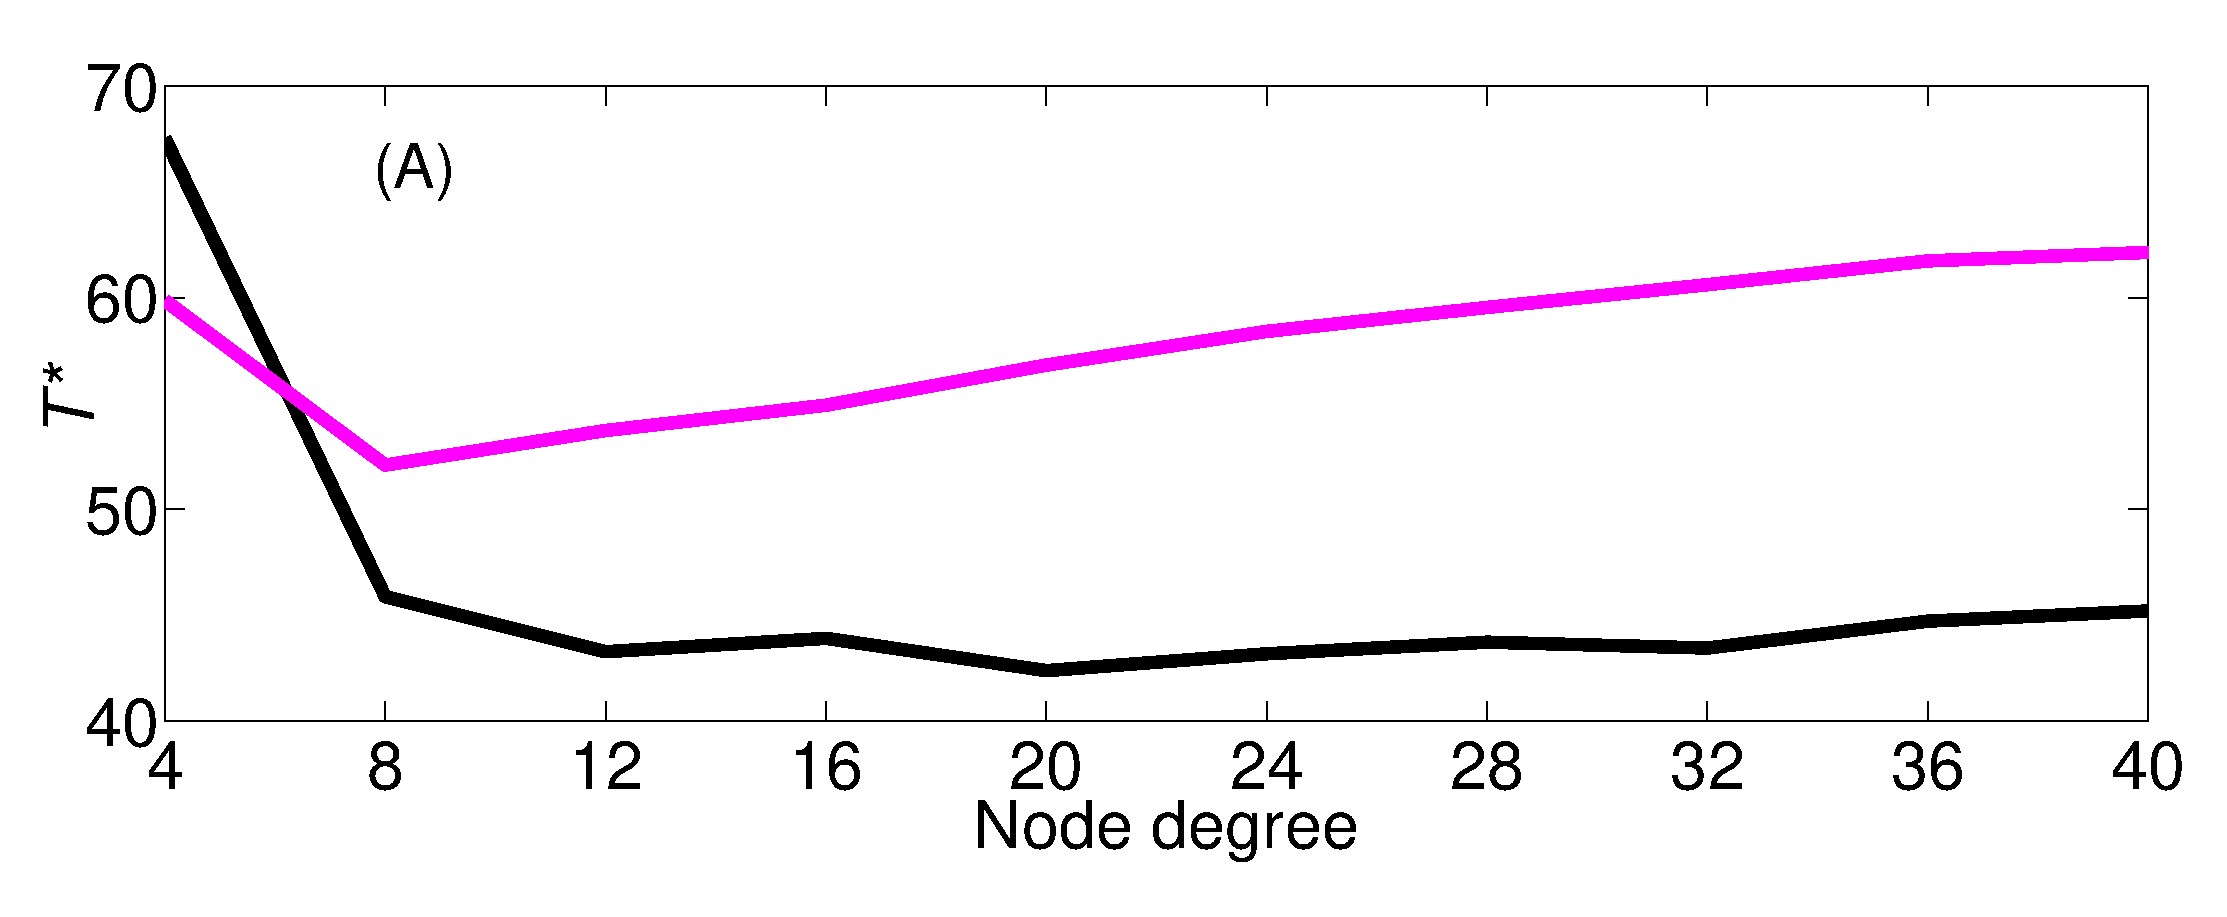
\includegraphics[scale=0.15]{figs1/random_graphs_delay.eps}
% % 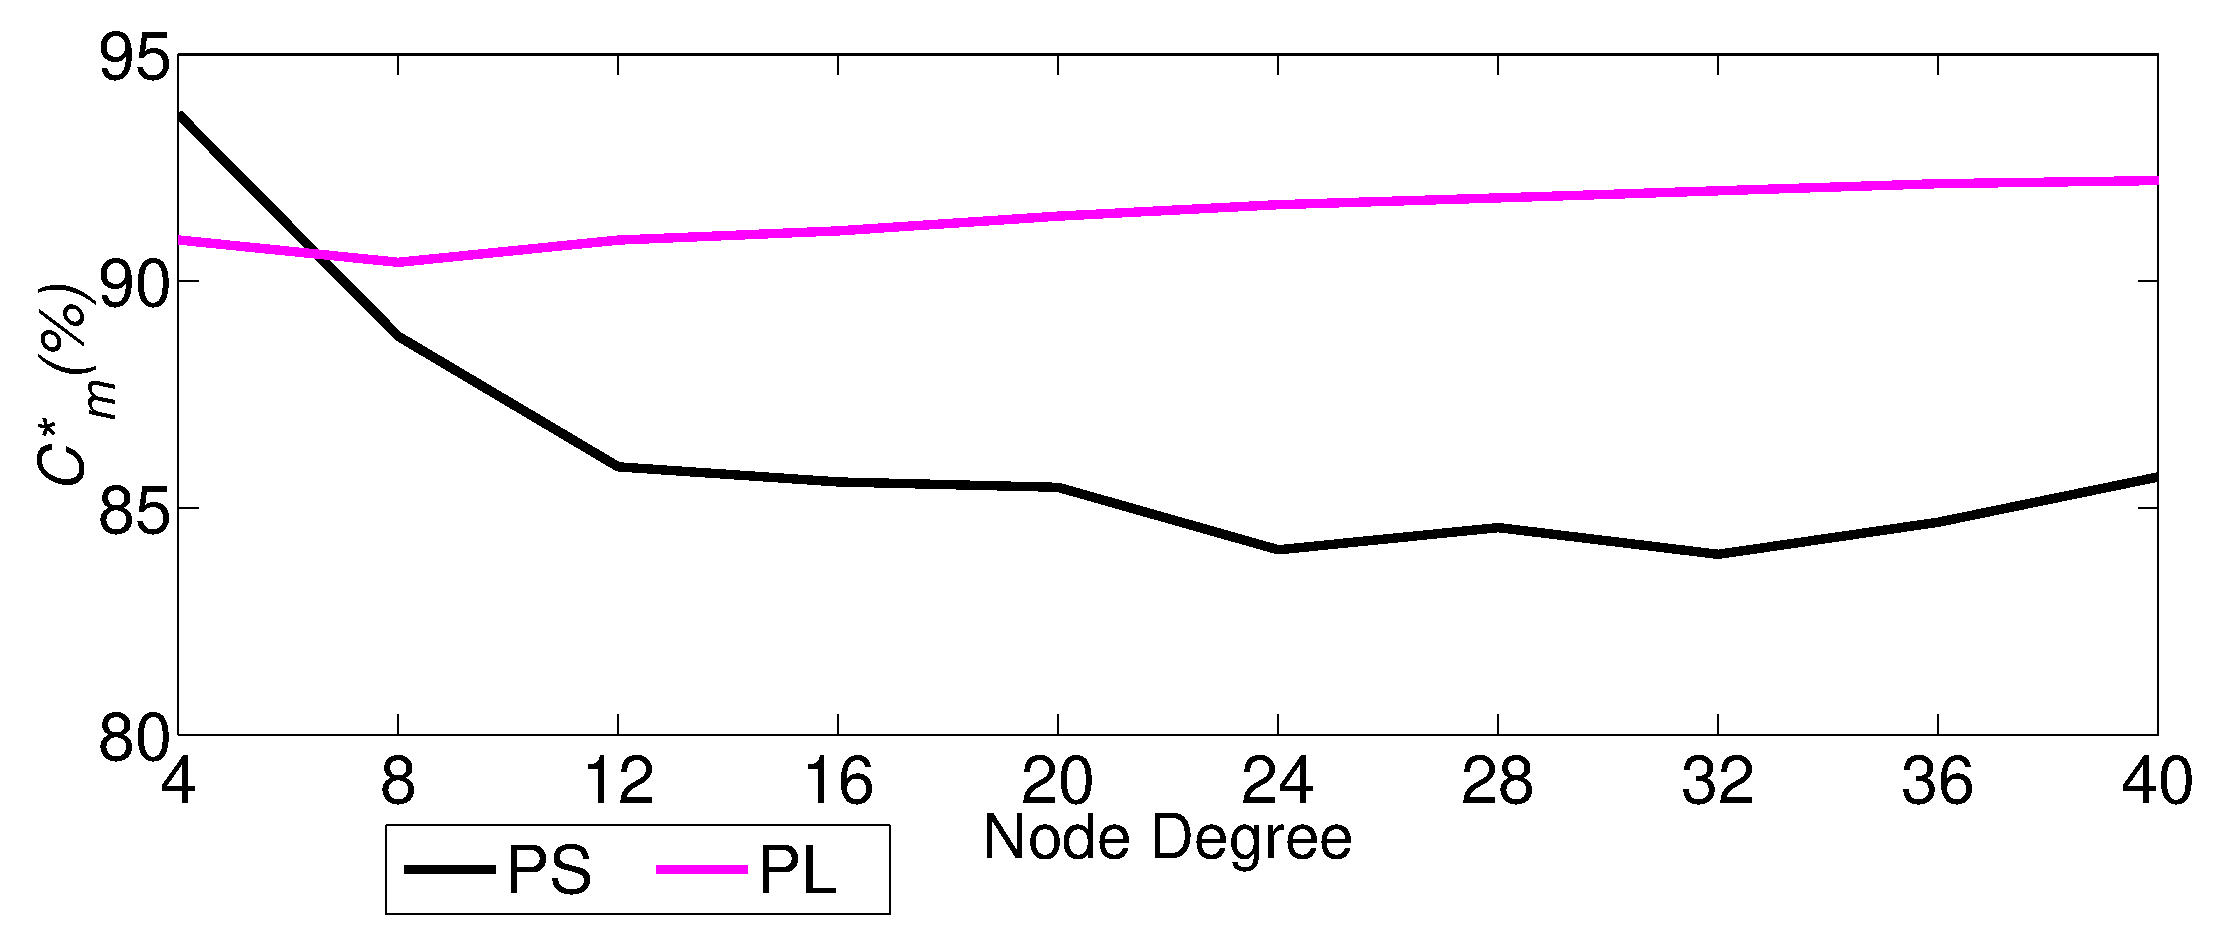
\includegraphics[scale=0.15]{figs1/random_graphs_wastage.eps}
% % \caption{(A) Broadcast time and (B) broadcast wastage versus average degree for B-P . The parameters values are $n=200, m=4, k=2$.\vspace{-3mm}}
% % \label{DiffTopologyGnp_N200_varyD_push_pull}
% % \end{figure}
% % 
% % \begin{figure}
% % \centering
% % \includegraphics[scale=0.4]{diagrams/M2final/DiffTopologyRegularTree_delay_cost_N200_m4_k2_varyD_ps_plRes.eps}
% % \caption{(A) Broadcast time and (B) broadcast wastage versus different values of $d$ for B-P. The parameters values are $n=200, m=4, k=2$.\vspace{-3mm}}
% % \label{DiffTopologyTree_N200_varyD_push_pull}
% % \end{figure}
% \vspace{-3mm}
%  \subsection{Random graph}
%  Here, we assume a random graph topology $G(n, p)$ where $n = 200$, $m = 4$ and $k=2$. Here we vary the probability $p$ of connection (equivalently the average degree $d$) from values ranging from 0.02 to 0.2 (the value of $d$ equivalently varies from 4 to 40) (see figure~\ref{DiffTopologyGnp_N200_varyD_push_pull}). Once again the same observation that both the broadcast time and the broadcast wastage become significantly low for a certain value of $d$ also hold in this case and for this value of $p$ the broadcast time is found to scale as $\log{(n)}$. 
% 
% Thus irrespective of the topology we are able to find a critical value of average degree for the network for which the dynamics becomes as fast as epidemic routing 
% even for the blind push case. Therefore for designing a topology for a network we recommend that the designers look for such a critical value of average degree 
% for which the dynamics becomes fast.
% 
% % \begin{figure}
% % \centering
% % 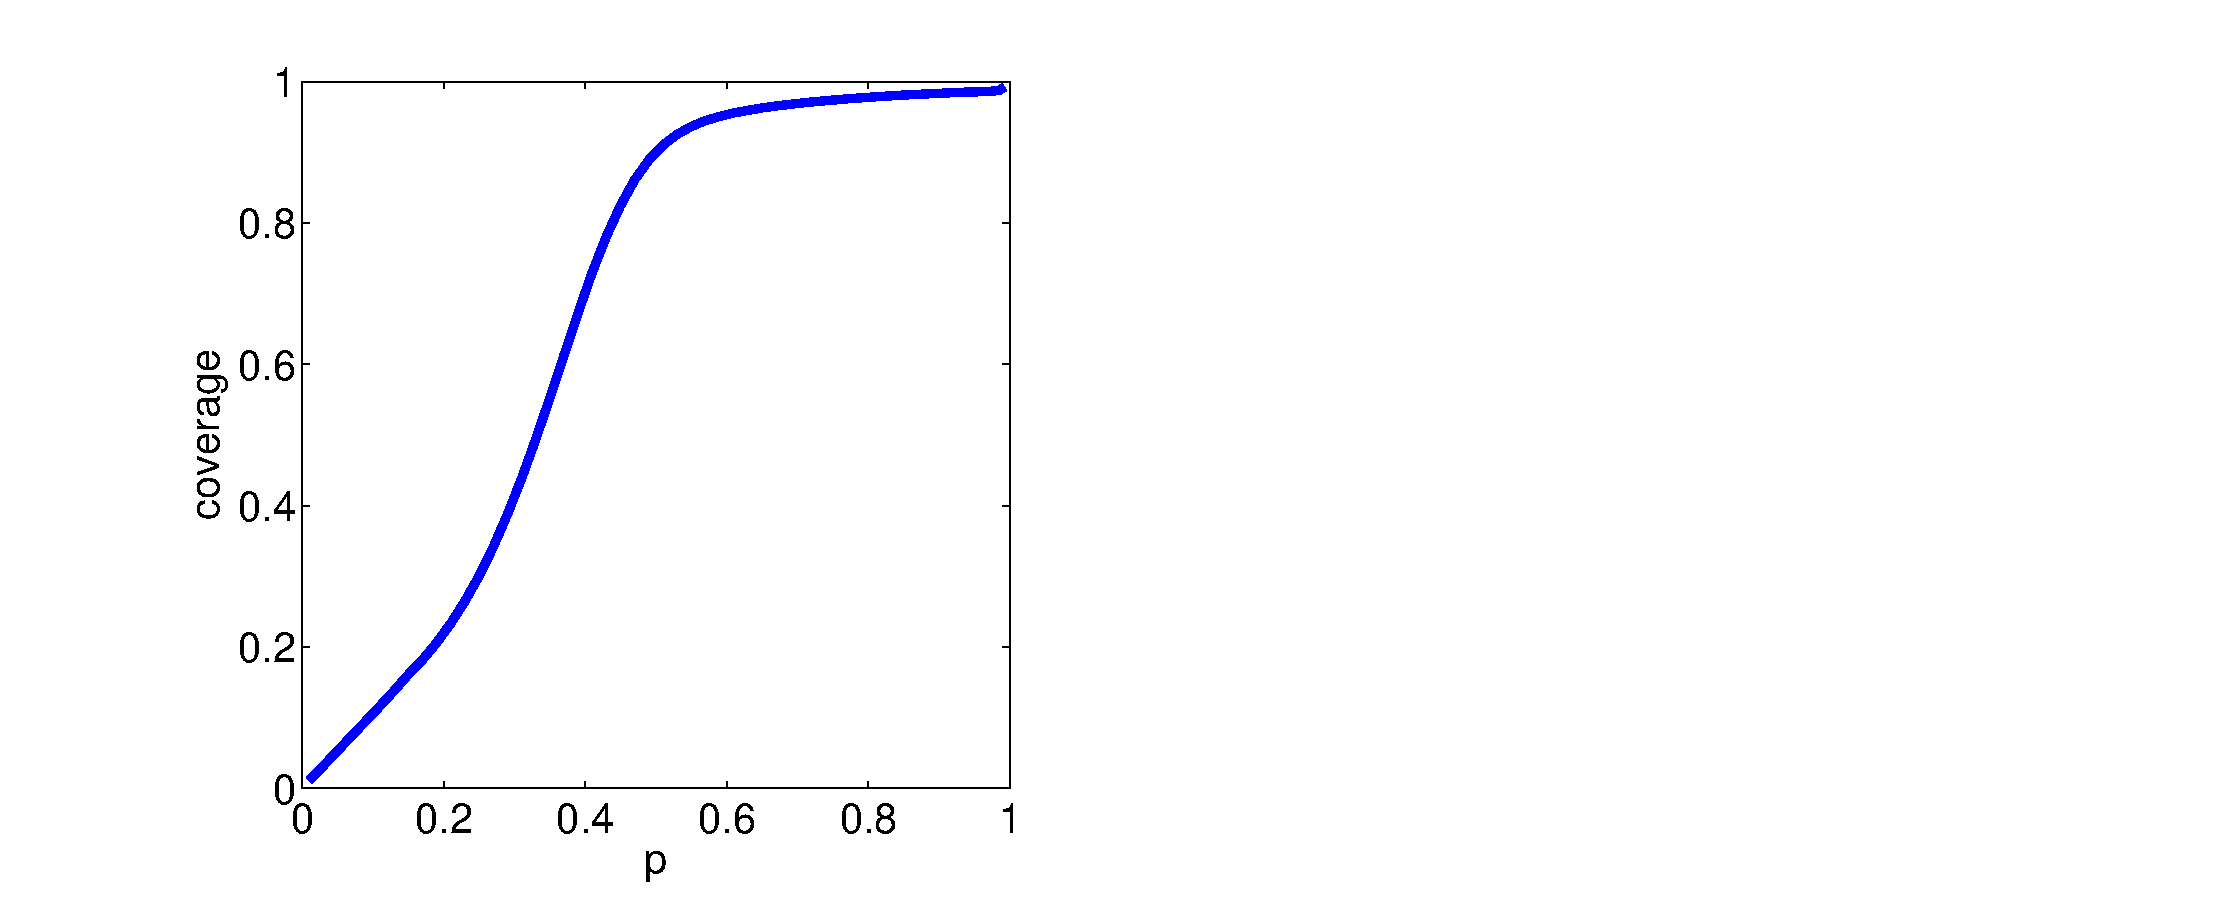
\includegraphics[scale=0.4]{figs1/pvsco.eps}
% % \caption{$p$ versus coverage for gnutella1 network, broadcast technique -- P-P-G \vspace{-3mm}}
% % \label{pcov}
% % \end{figure}

% Since the value of the critical average degree is found to be on the lower side, we performed simulations on sparser variants of the real traces (used previously) 
% and observed that broadcast time reduces even for the B-P. We considered each gnutella snapshot and randomly removed some of the edges such that the 
% network remains connected while producing a sparser variant. From figure ~\ref{gnutellasparse} we observe that the broadcast time reduces significantly 
% in case of the sparser variants in comparison to the original network. 
% Hence, while designing a network it is advisable to keep the network sparse rather than creating unnecessary connections between the nodes. 
% This, as our results indicate, should lead to a faster dissemination of messages.
% \begin{figure}
% \centering
% \includegraphics[scale=0.15]{figs1/random_graphs_delay1.eps}
% \includegraphics[scale=0.15]{figs1/random_graphs_wastage1.eps}
% \caption{(A) Broadcast time and (B) broadcast wastage versus average degree for B-P . The parameters values are $n=200, m=4, k=2$.\vspace{-3mm}}
% \label{DiffTopologyGnp_N200_varyD_push_pull}
% \end{figure}

\begin{figure}
\centering
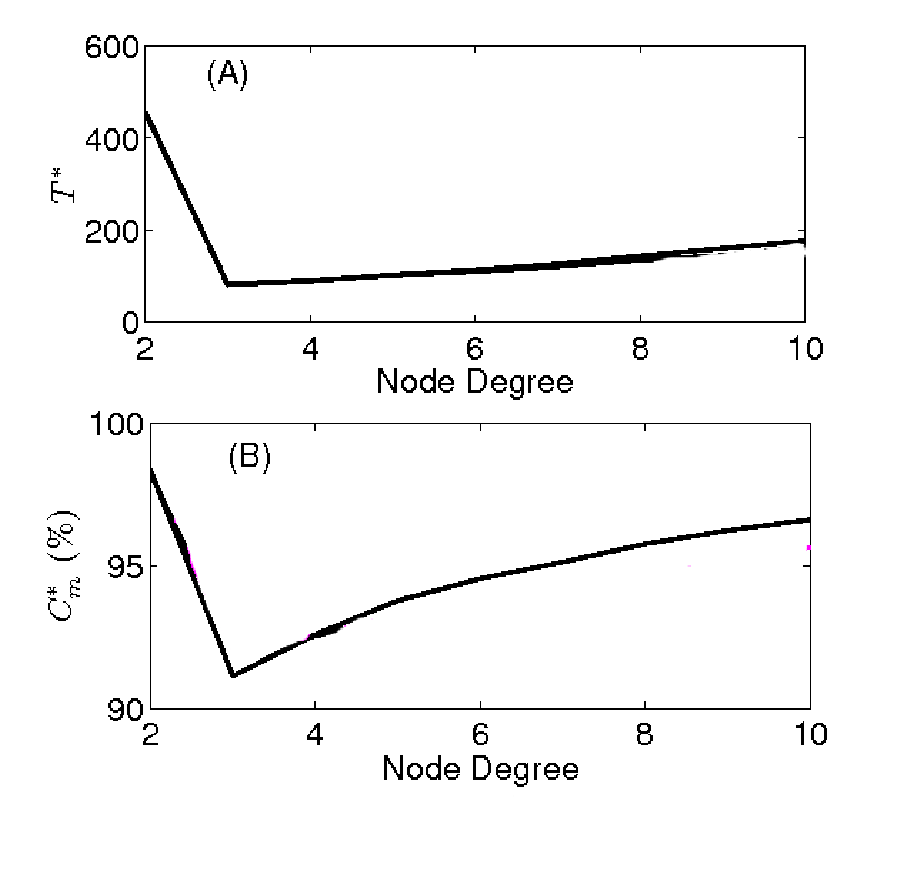
\includegraphics[scale=0.4]{./texfiles/Chapter_3/netsci/figs1/DiffTopologyRegularTree_delay_cost_N200_m4_k2_varyD_ps_plRes1.eps}
\caption{(A) Broadcast time and (B) broadcast wastage versus different values of $d$ for B-P. The parameters values are $n=200, m=4, k=2$.}
\label{DiffTopologyTree_N200_varyD_push_pull}
\end{figure}
%\subsection{Random graph}
%In this section, we assume a random graph topology $G(n, p)$ where $n = 200$, $m = 4$ and $k=2$. Here we vary the probability $p$ of connection (equivalently the average degree $d$) from values ranging from 0.02 to 0.2 (the value of $d$ equivalently varies from 4 to 40) (see figure~\ref{DiffTopologyGnp_N200_varyD_push_pull}). Once again the same observation that both the broadcast time and the broadcast wastage become significantly low for a certain value of $d$ also hold in this case and for this value of $p$ the broadcast time is found to scale as $\log{(n)}$. 

\begin{figure}
\centering
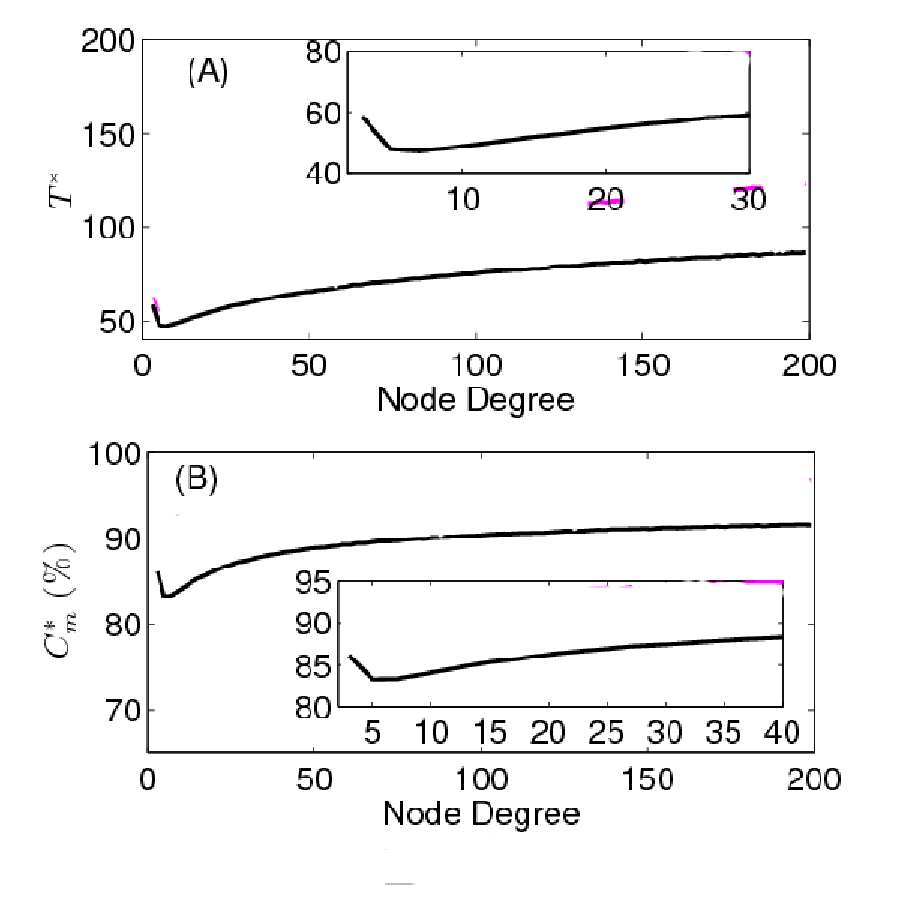
\includegraphics[scale=0.39]{./texfiles/Chapter_3/netsci/figs1/DiffTopology_varyN200_varyD_push_pullRes_m4_k21.eps}
\caption{(A) Broadcast time and (B) broadcast wastage versus different values of $d$ for B-P technique. The parameters values are $n=200, m=4, k=2$. The inset in both the figures show the metrics of interest for the first few values of $d$ to indicate the critical $d$ more appropriately.\vspace{-3mm}}
\label{DiffTopologyGraph_N200_varyD_push_pull}
\end{figure}

\begin{figure}
\centering
\includegraphics[scale=0.21]{./texfiles/Chapter_3/netsci/figs1/random_graphs_delay1.eps}
\includegraphics[scale=0.21]{./texfiles/Chapter_3/netsci/figs1/random_graphs_wastage1.eps}
\caption{(A) Broadcast time and (B) broadcast wastage versus average degree for B-P . The parameters values are $n=200, m=4, k=2$.}
\label{DiffTopologyGnp_N200_varyD_push_pull}
\end{figure}
\begin{figure}
\centering
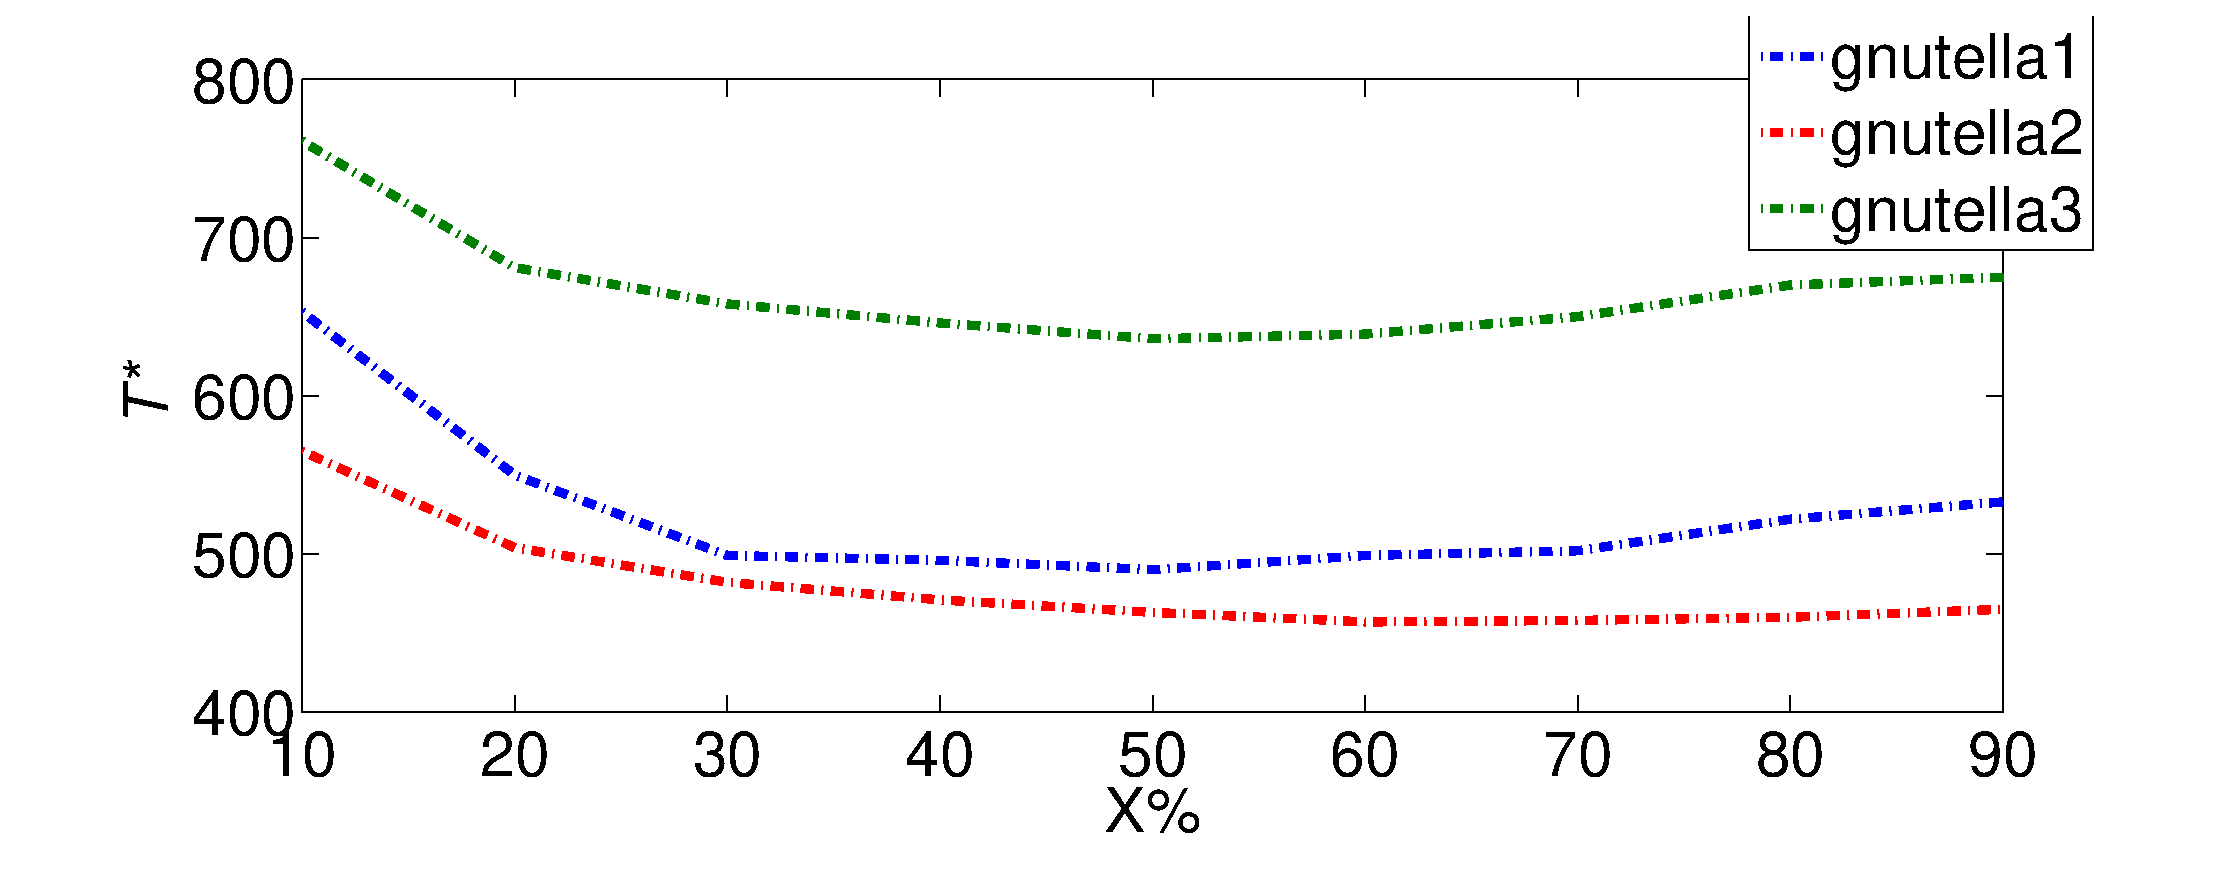
\includegraphics[scale=0.21]{./texfiles/Chapter_3/netsci/figs1/xperbt.eps}
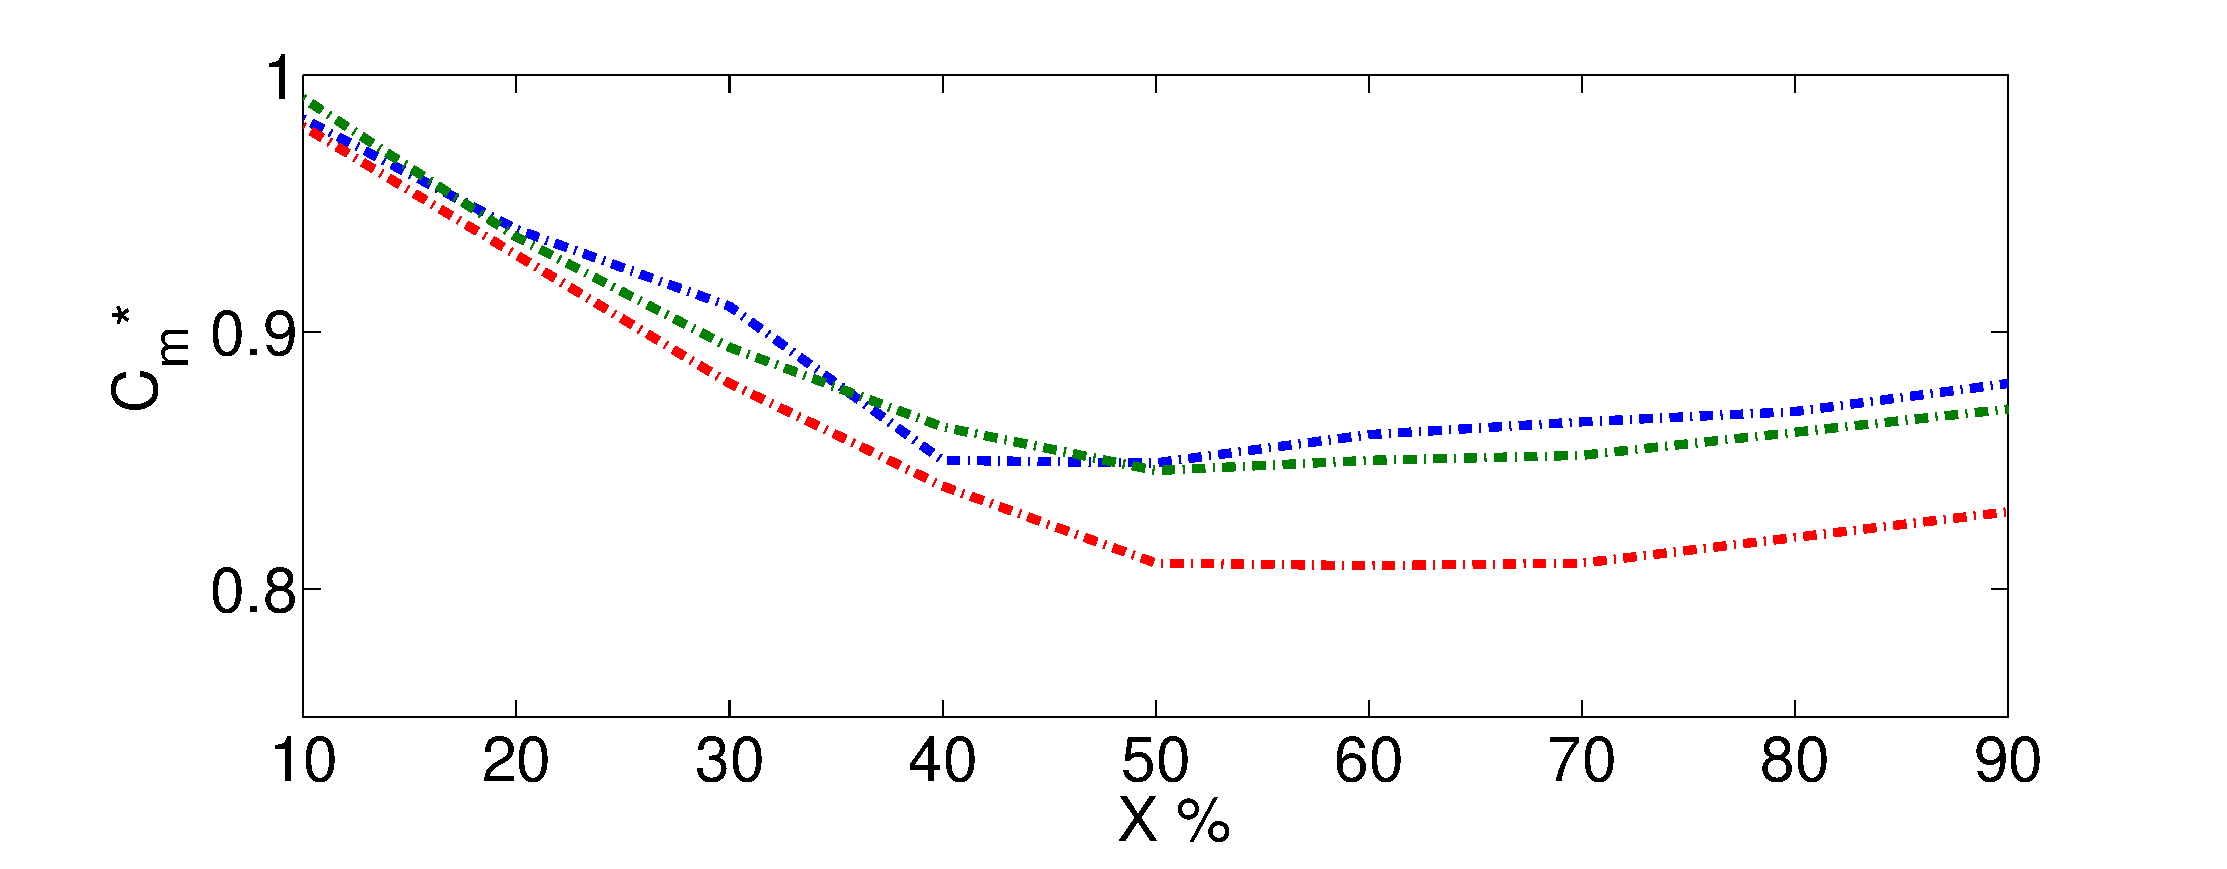
\includegraphics[scale=0.21]{./texfiles/Chapter_3/netsci/figs1/xperwa.eps}
\caption{Average broadcast time and wastage versus x for gnutella1,gnutella2 and gnutella3}
\label{ps_bt}
\end{figure}

% \begin{figure}
% \centering
% 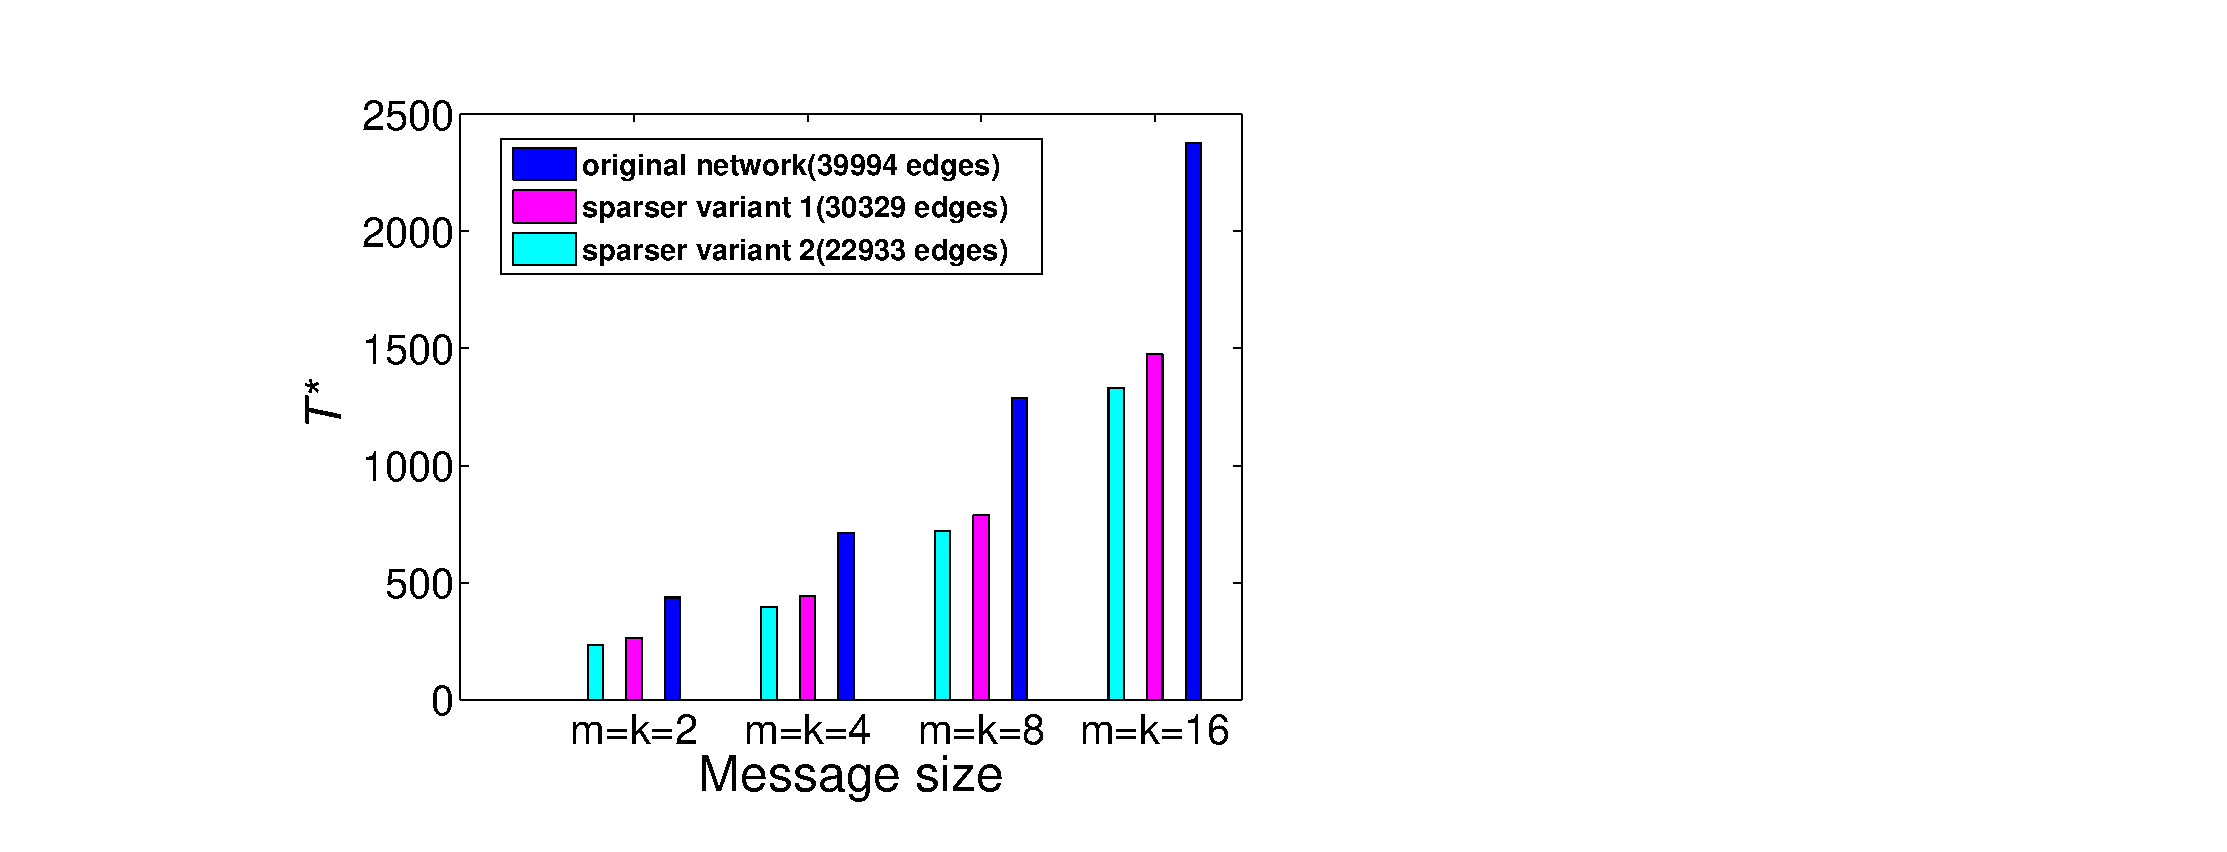
\includegraphics[scale=0.25]{figs1/gnutella1.eps}
% 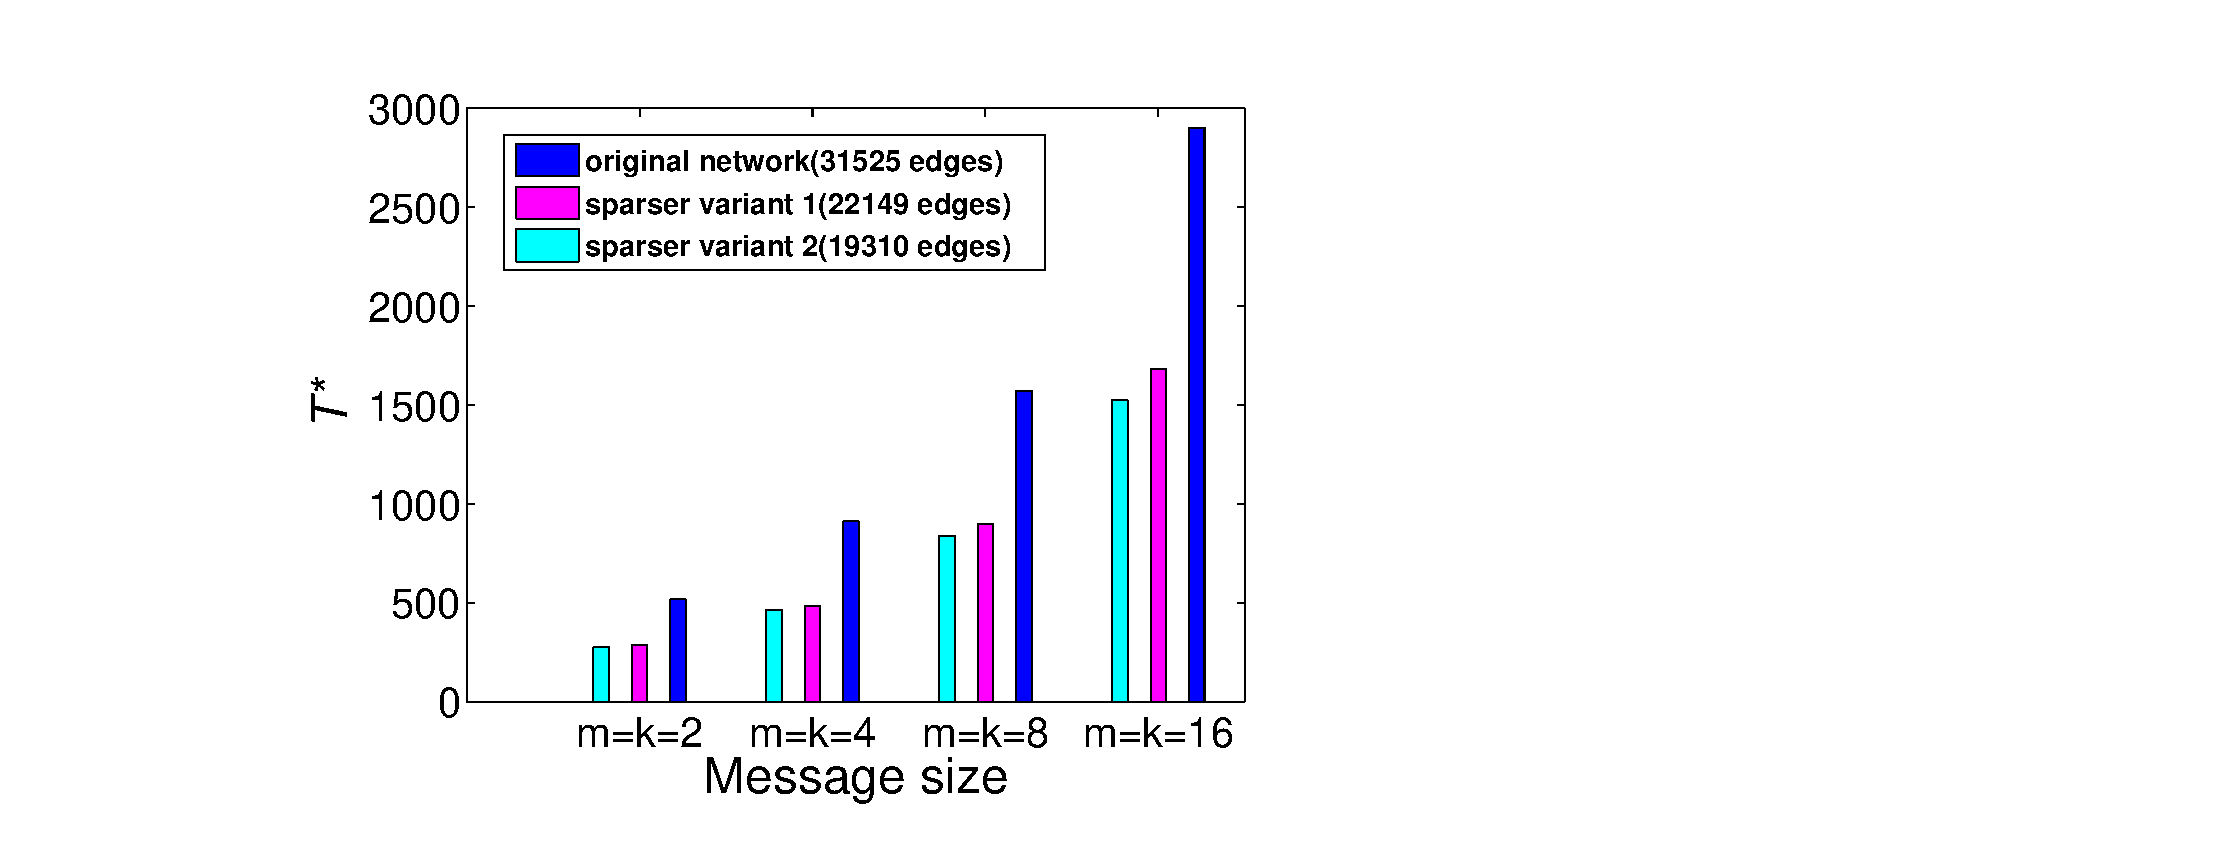
\includegraphics[scale=0.25]{figs1/gnutella2.eps}
% \caption{Broadcast time for the gnutella snapshots and their sparser variants versus different values of message sizes for gnutella1 and gnutella2\vspace{-3mm}}
% \label{gnutellasparse}
% \end{figure}
% \medskip
